\documentclass{article}
% The documentclass command is required in LaTeX


% I CAN TYPE CHANGES WITHOUT A MOUSE  
% I am making changes to the LaTeX code for this project
% I got the created project from GitHub
% I can escape editing with OPTION + TAB
            
% Packages are our toolboxes and are defined at the 
% top of our sourcecode in this preamble.
\usepackage[utf8]{inputenc}

%%%%%%%% PACKAGES
\usepackage{amsmath}  % displaying math equations
\usepackage{verbatim} % comment blocks
\usepackage{hyperref} % hyperlinks
\usepackage[version=4]{mhchem} % chemistry formulas
\usepackage{chemfig} % chemistry 2D diagrams

\usepackage{graphicx} %package to manage images
\graphicspath{ {./images/} }
\usepackage[rightcaption]{sidecap}
\usepackage{wrapfig} % wrapping figures
\usepackage{apacite} % APA citation style bibliOgraphy
% preamble global changes
%make a change
    
    
\usepackage{microtype}
% \usepackage[a4paper, total={6.5in, 9in}]{geometry} % control text space
\usepackage{helvet}

% In the body of the document, we will print these with
% the command \maketitle
\title{\LaTeX for Science and Math}
\author{Brandeis Library Data Services }
\date{October 26, 2020}


% The Begin and End document commands are required
% They define the body of the text.
\begin{document}
% THE BODY OF THE DOCUMENT BEGINS HERE


\maketitle

\tableofcontents

\pagebreak

\section{Introduction to Structure}
\subsection{I can add subsections}
\subsubsection{And sub sub section, etc.}

Lorem ipsum dolor sit amet, consectetur adipiscing elit. Fusce risus 
urna, finibus at augue luctus, mattis mollis tellus. Aliquam consequat 
accumsan magna sit amet vestibulum. Cum sociis natoque penatibus et 
magnis dis parturient montes, nascetur ridiculus mus. Maecenas ut 
pellentesque mauris. Nulla ac dolor at leo hendrerit interdum. Etiam 
vulputate posuere nisi in tincidunt. Sed non scelerisque purus. Phasellus 
efficitur faucibus nisl, eget posuere urna. Phasellus tincidunt dui 
lacus, in semper nulla volutpat eget. Pellentesque habitant morbi 
tristique senectus et netus et malesuada fames ac turpis egestas. 
Suspendisse nibh massa, rhoncus aliquam mattis in, ultrices eu urna. 
Vivamus in accumsan erat.

\section{Comments and Formatting}
% Percentage signs indicate single line comments
% Comments are not executed
% They do not appear in the output.

% We can also comment out entire blocks like this:
\begin{comment} %usepackage{verbatim} for comment blocks
    \section{Unfinished Results}
    I don't have to share everything.
    I can have writing that I save for later.
\end{comment}

And of course we have all the typical functionality of \textbf{bold fonts}, \textit{italizied} fonts, and changing font justification.  The global changes we want to make in terms of fonts and style are done in the \emph{preamble} above the document body (denoted by the command begin\{document\} ).

Bullet Point Lists
\begin{itemize}
    \item Apples
    \item bananas
    \item $E=mc^2$
\end{itemize}

Enumerated (Numbered) Lists
\begin{enumerate}
    \item Apples
    \item bananas
    \item $E=mc^2$
\end{enumerate}

Don't forget to check out the Error Log when you recompile.  It will give suggestions about debugging and let you know what lines in your source code have errors.  Google, Stackoverflow, and your friendly Data Analysis Specialist at the Library (that's me) are always happy to help.


\section{Math}  
There is great Power in the handling of symbols and formulas for LaTeX.  We can display mathematical expressions and symbols "inline" in the text like this $\frac{1}{2}$ with \$ signs, or with square brackets.

We need to usepackage amsmath for flexibility in displayed (not in-line) equations and how they are aligned.  

\LaTeX has symbols for operators $\times \dot \div$, Greek letters $\alpha \beta \Delta \Gamma$, and arrows $\Rightarrow$.
\href{https://www.overleaf.com/learn/latex/List_of_Greek_letters_and_math_symbols}{List of Greek Letters and Math Symbols}


\subsection{Inline vs. display math mode}
The mass-energy equivalence is described by the famous equation \[ E=mc^2 \]
discovered in 1905 by Albert Einstein. 
In natural units ($c = 1$), the formula expresses the identity
\begin{equation}
E=m
\end{equation}


\begin{equation}
\begin{split}. %notice the equation is aligned at the equals sign
A & = \frac{\pi r^2}{2} \\
 & = \frac{1}{2} \pi r^2
\end{split}
\end{equation}

\subsection{Writing a single equation}
We can use the command begin with argument equation from the amsmath package.  Notice, if we add an asterisk to the argument, the equation is not numbered.
\begin{equation} 
e^{\pi i} + 1 = 0
\end{equation}
The above equation is numbered. 
\begin{equation*}
e^{\pi i} + 1 = 0
\end{equation*}
The above equation is not numbered.
\begin{equation} \label{eu_eqn}
e^{\pi i} + 1 = 0
\end{equation}
The above equation is numbered and referenced with the special label $eu_eqn$.  I can call this as a clickable reference in the text below.

The beautiful equation \ref{eu_eqn} is known as the Euler equation

\subsection{Displaying long equations}
We can use multline from amsmath and two slashes for a break to split up long equations.
\begin{multline*}
p(x) = 3x^6 + 14x^5y + 590x^4y^2 + 19x^3y^3 \\  %the two slashes break line
- 12x^2y^4 - 12xy^5 + 2y^6 - a^3b^3
\end{multline*}


\subsection{Aligning several equations}
We can use align from amsmath to align systems of equations at their equals sign.  Double slashes denote a line break.
\begin{align*} 
2x - 5y &=  8 \\ 
3x + 9y &=  -12
\end{align*}


\subsection{Matrices}
The package amsmath supports matrices.  Below is an example of a matrix with square brackets.  Columns are separated by the ampersand.  Rows are separated by the double slash.  See \href{https://www.overleaf.com/learn/latex/Matrices}{Overleaf Overview of Matrices} for more examples.
\begin{equation}
\begin{bmatrix}
1 & 2 & 3\\
a & b & c
\end{bmatrix}
\end{equation}

\subsection{Typing superscripts and subscripts}
Underscores and carets are used.  
Superscripts and subscripts can also be used to assign limits next to integrals as in the example below.
\begin{equation*}
    \int_0^\infty e^{-x^2} dx=\frac{\sqrt{\pi}}{2}
\end{equation*}

Notice we can also use the limits command to bring the (sub-scripted and super-scripted) limits of integration above and below the integration sign.
\[ \int\limits_0^1 x^2 + y^2 \ dx \]
\[ a_1^2 + a_2^2 = a_3^2 \]

Curly brackets are needed if more than one character is in sub or superscripts.
\[ x^{2 \alpha} - 1 = y_{ij} + z_{ij}  \]
\[ (a^n)^{r+s} = a^{nr+ns}  \]

\subsubsection{Operators using subscripts}
\[ \sum_{i=1}^{\infty} \frac{1}{n^s} 
= \prod_p \frac{1}{1 - p^{-s}} \]

\subsection{Parentheses and Brackets}
Notice the size of brackets scales automatically.  We can define left and right brackets, but we also have control on size if we need it.  See a great Overleaf overview \href{https://www.overleaf.com/learn/latex/Brackets_and_Parentheses}{here.}

\[ F = G \left( \frac{m_1 m_2}{r^2} \right) \]

\subsection{Typing fractions}
Fractions can be used alongside the text, for 
example \( \frac{1}{2} \), and in a mathematical 
display style like the one below:

\[\frac{1}{2}\]

The fractions can be nested

\[ \frac{1+\frac{a}{b}}{1+\frac{1}{1+\frac{1}{a}}} \]


\section{Chemistry}
See more information in Overleaf documentation on \href{https://www.overleaf.com/learn/latex/Chemistry_formulae}{Chemistry formula.} and in the Chemistry diagrams section of the \href{https://en.wikibooks.org/wiki/LaTeX/Chemical_Graphics}{LaTeX wikibook.}

\subsection{Chemical formulas}

Writing formulas with \textbf{mhchem}
Notice the command ce (for chemical equation) has an easier syntax than math mode, and chemical symbols are not italicized as math variables are.  Underscores are not needed in basic compound writing. For example:
\ce{3H2O}

\ce{SO4^2-} %sulfate!

\ce{1/2 H2O}

\ce{H2_{(aq)}}

\ce{^{227}_{90}Th+}

\ce{CO2 + C -> 2CO}


\subsection{2D diagrams}
Writing chemical formulas with package chemfig

\chemfig{0=H}

% you can define angles to draw bonds between molecules
\chemfig{A-[:50]B-[:-25]C}

% Syntax to draw rings
\chemfig{A*5(-B=C-D-E=)}


\section{Graphics}
We need to use the package \textit{graphicx} to manage packages.  Supported formats include eps, pdf, jpg, and png.  

Create an images folder and upload the image files to it.



Example 1.  Simplest example of including a picture with no extra parameters.
We can add some vertical space with vspace.
\vspace{1.5cm}

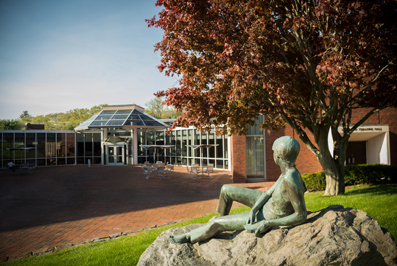
\includegraphics{library}

Note: The file extension is allowed to be included, but if it is omitted \LaTeX will search for all the supported formats.


\newpage
% --------

Example 2. Scaling and image

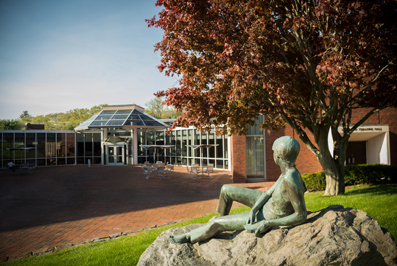
\includegraphics[scale=0.5]{library}

\vspace{1.5cm}

% --------

Example 3. Setting specific width and height. We can specify inches (in), centimeters (cm), pixels (px)

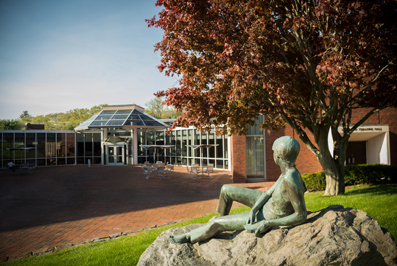
\includegraphics[width=5in, height=4in]{library}

\newpage

% --------

Example 4. Importing Images example, rotating

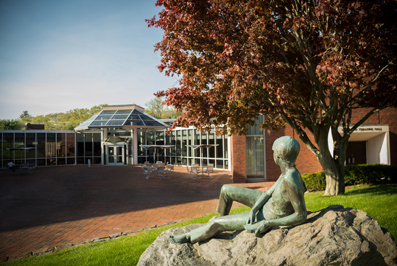
\includegraphics[scale=.3, angle=45]{library}

% --------

Example 5. Importing Images example, alternative units

\vspace{1.5cm}

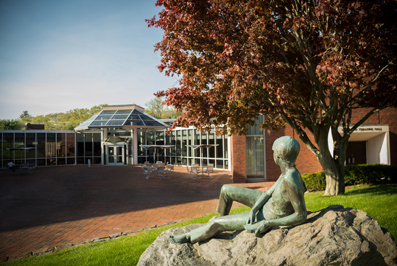
\includegraphics[width=\textwidth]{library}

\newpage

% --------
Example 6. Example, placing images
In the next example the figure will be positioned right below this sentence.

\begin{figure}[h]
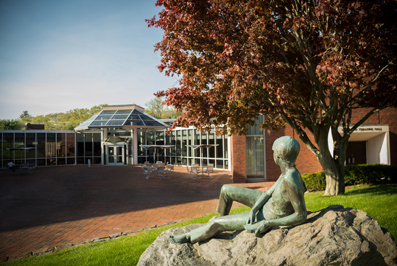
\includegraphics[width=8cm]{library}
\end{figure}

\newpage

% --------
Example 7. The image will be at the top as designated by t

\begin{figure}[t]
\centering
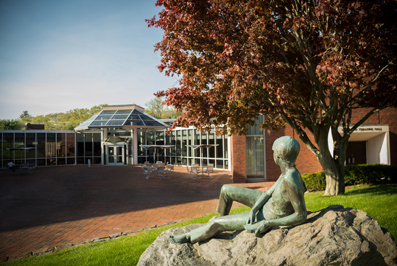
\includegraphics[width=8cm]{library}
\end{figure}

\newpage

% --------
Example 8. Floating pictures. Text wrapping the figure.  r is for right, use l for left alignment.

\begin{wrapfigure}{r}{0.25\textwidth} %this figure will be at the right
    \centering
    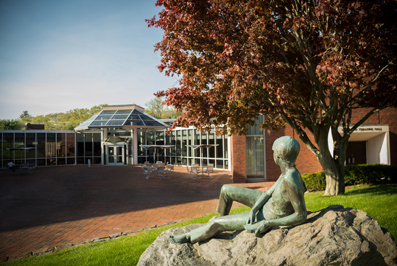
\includegraphics[width=0.4\textwidth]{library}
\end{wrapfigure}

\vspace{1.2cm}

Lorem ipsum dolor sit amet, consectetur adipiscing elit. Fusce risus 
urna, finibus at augue luctus, mattis mollis tellus. Aliquam consequat 
accumsan magna sit amet vestibulum. Cum sociis natoque penatibus et 
magnis dis parturient montes, nascetur ridiculus mus. Maecenas ut 
pellentesque mauris. Nulla ac dolor at leo hendrerit interdum. Etiam 
vulputate posuere nisi in tincidunt. Sed non scelerisque purus. Phasellus 
efficitur faucibus nisl, eget posuere urna. Phasellus tincidunt dui 
lacus, in semper nulla volutpat eget. Pellentesque habitant morbi 
tristique senectus et netus et malesuada fames ac turpis egestas. 
Suspendisse nibh massa, rhoncus aliquam mattis in, ultrices eu urna. 
Vivamus in accumsan erat.

\newpage

% --------

Example 9. Captioning

\begin{figure}[h]
\caption{Example of a caption}
\centering
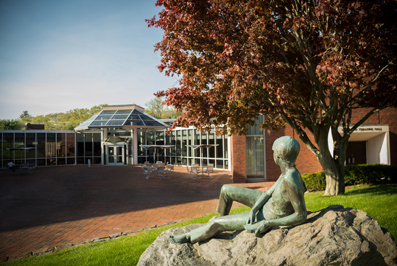
\includegraphics[width=0.6\textwidth]{library}
\end{figure}

% --------

\vspace{1.5cm}

Example 10. Caption next to the figure using the sidecap argument SCfigure
\begin{SCfigure}[0.5][h]
\caption{Using again the photo of the library. 
         This caption will be on the right}
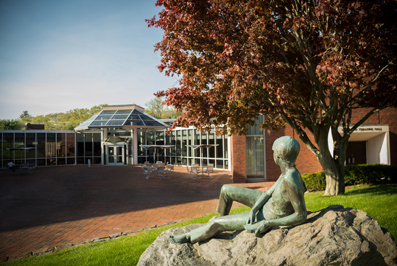
\includegraphics[width=0.6\textwidth]{library}
\end{SCfigure}

\newpage

% --------
Example 11. Labeling and referencing example
\begin{figure}[h]
    \centering
    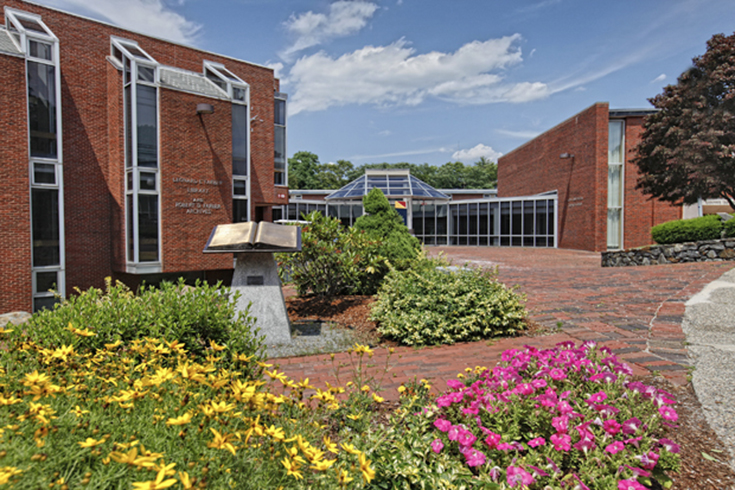
\includegraphics[width=0.5\textwidth]{flowers}
    \caption{The library in springtime.}
    \label{fig:library}
\end{figure}

As you can see in the figure \ref{fig:library}, the library is in the sunshine. Also, in the page \pageref{fig:library} is the same example.

\vspace{1.5cm}

% --------
Example 12. Let's generate the images index.
\begin{figure}[h]
    \centering
    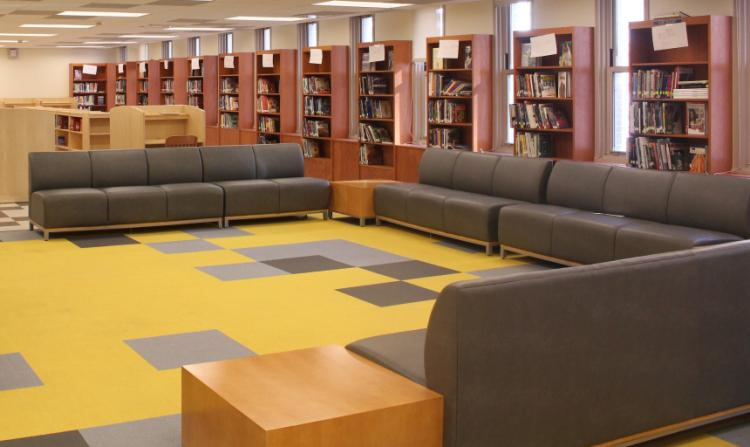
\includegraphics[width=0.5\textwidth]{stacks}
    \caption{An interior view}
    \label{fig:inside}
\end{figure}

\newpage

%Generating a list of figures
\listoffigures

% -----------------------------------------------
\section{Tables}
You can use the tabular argument to make tables in \LaTeX.  Use | and hline to add vertical and hosizontal lines to tables in \LaTeX.  More detailed examples are in the \href{https://www.overleaf.com/learn/latex/Tables}{Overleaf help.}

\begin{center}
\begin{tabular}{ c | c  c }
 cell1 & cell2 & cell3 \\ 
 \hline
 cell4 & cell5 & cell6 \\  
 cell7 & cell8 & cell9    
\end{tabular}
\end{center}


\section{Bibliographies}
You can download BibTex format from Zotero, Endnote, Brandeis Library OneSearch, and other citation management tools.  To add APA citations, we use the apacite package and cite command with the reference as the argument.  The reference label is the first part of the .bib entry for your resource.  For example,the Intro to LaTeX research guide \cite{ClairePontbriand2019ItL} lists resources. 

We use the bibliography command where we want the references listed.  
\bibliographystyle{apacite}
\bibliography{bibtex.bib}

\section{The Preamble}
Add the package microtype in your preamble. These changes are subtle modifications on the inter word spacing and kerning. It tends to make your document look just a little bit better. 

We can use the geometry package to manage margins.

Read more about \href{https://www.overleaf.com/learn/latex/Page_size_and_margins}{fine-tuning page size and margins.}

{\fontfamily{phv}\selectfont
In \LaTeX the default font typeface is the \textbf{Computer Modern} family. You can change this font typeface for another that better suits your style.
See more about typefaces \href{https://www.overleaf.com/learn/latex/Font_typefaces}{here} and in the \href{https://tug.org/FontCatalogue/}{LaTeX Font Catalogue}

This is Helvetica	(helvet	phv)
}

\section{Resources}
\begin{itemize}
    \item \href{https://stackoverflow.com/}{Stackoverflow}
    \item \href{https://en.wikibooks.org/wiki/LaTeX}{LaTeX in Wikibooks}
    \item \href{https://www.ctan.org/pkg/brandeis-dissertation?lang=en}{Class for Brandeis Dissertations}
    \item \href{https://tex.stackexchange.com/questions/183358/how-to-convert-a-google-docs-document-to-latex}{Stackexchange thread about how to convert from docs to \LaTeX}
    \item \href{https://pandoc.org/}{Pandoc - a universal document converter}
    \item \href{}{}
\end{itemize}


% END DOCUMENT IS REQUIRED COMMAND
\end{document}
                    